% Marc teòric.
%

Aquest apartat estableix la base teòrica necessària per comprendre l'evolució dels contenidors i l'impacte arquitectònic que els diferents models d'orquestració exerceixen sobre l'execució de càrregues d'Intel·ligència Artificial en entorns amb recursos limitats.

\section{Tecnologies de Virtualització i Contenidors}
Els contenidors formen una tecnologia de virtualització a nivell de sistema operatiu que permet empaquetar una aplicació i totes les seves dependències dins d'una unitat estandarditzada. A diferència de les màquines virtuals, els contenidors comparteixen el nucli (\textit{kernel}) del sistema amfitrió, fet que els dota d'una lleugeresa notable, d'un inici ràpid i d'una gran eficiència en l'ús de CPU i memòria.

\textbf{Arquitectures amb dimoni i sense dimoni (\textit{Daemonless}):}
Tradicionalment, motors com Docker s'han basat en un dimoni (\textit{daemon}), un procés central en segon pla —generalment executat amb privilegis d'administrador— que gestiona tot el cicle de vida dels contenidors. Si aquest dimoni falla, s'atura la totalitat del sistema. Com a evolució tecnològica, sorgeix Podman, un motor de contenidors sense dimoni que interactua directament amb el nucli mitjançant processos independents \cite{podman_pod}, millorant així la seguretat, reduint el consum en repòs i integrant-se de manera natural amb el sistema operatiu.

\section{L'Evolució de l'Orquestració i el biaix a l'\textit{Edge}}
L'orquestració s'encarrega d'automatitzar el desplegament, l'escalabilitat i la resiliència de múltiples contenidors. Històricament, l'evolució d'aquests sistemes a la indústria ha passat per tres fases clarament diferenciades:  

\begin{enumerate}
    \item \textbf{La consolidació de Kubernetes al \textit{Cloud}:}
    Durant els inicis de la contenerització, diverses tecnologies (com ara Docker Swarm o Apache Mesos) van competir per liderar el sector. Cap al 2018, Kubernetes es va imposar de manera absoluta, esdevenint l'estàndard indiscutible per a la gestió de grans centres de dades (\textit{Cloud}).

    \item \textbf{El dogma d'un Kubernetes cada vegada més lleuger:}
    Quan va sorgir la necessitat d'estendre la contenerització cap als extrems de la xarxa (\textit{Edge Computing}), el sector va adoptar una visió reduccionista: l'única via viable consistia a ``encongir'' Kubernetes. Els esforços d'enginyeria es van centrar a retallar components per encabir l'orquestrador en maquinari modest, donant lloc a distribucions com K3s o MicroK8s. Malgrat tot, aquestes solucions mantenien inalterable l'arquitectura base: un procés resident (\texttt{kubelet}) per node i complexes xarxes virtuals internes (SDN).  

    \item \textbf{El buit metodològic:}
    Aquesta tendència va consolidar una falsa dicotomia en l'àmbit pràctic:  
    \begin{itemize}
        \item O bé s'assumia la penalització permanent de memòria i CPU d'un Kubernetes lleuger per mantenir actiu el clúster.  
        \item O bé s'optava per l'ús de contenidors aïllats (\textit{standalone}), sacrificant completament la gestió centralitzada i la capacitat d'autorecuperació davant d'errors.
    \end{itemize}
\end{enumerate}

\section{L'Enfocament Natiu: Systemd, Quadlets i Ansible}
Per superar aquesta limitació, s'ha impulsat una alternativa tècnica —promoguda inicialment per Red Hat— que proposa un canvi de paradigma: en comptes d'afegir un agent extern (\texttt{kubelet}) que consumeixi recursos de manera constant en un dispositiu limitat, per què no delegar aquesta funció en el gestor de processos natiu que Linux ja incorpora per defecte?  

Aquí és on entra Systemd, el sistema d'inicialització estàndard de Linux, dissenyat per arrencar serveis i reiniciar-los de forma gairebé instantània si fallen. Si bé anteriorment integrar contenidors amb Systemd exigia redactar fitxers de servei complexos (\textit{Legacy}), avui dia s'empren els \textit{Quadlets} \cite{podman_systemd_unit}, una utilitat nativa de Podman que permet definir els contenidors de manera declarativa i traduir-les automàticament a serveis gestionats directament pel \textit{kernel}.

\textbf{La simulació d'un orquestrador mitjançant Ansible:}
Com que Systemd i Podman operen de manera aïllada a cada màquina, l'arquitectura s'estén mitjançant Ansible, una eina d'automatització sense agents. Combinant aquestes tecnologies, és possible replicar l'estabilitat d'un orquestrador sencer estalviant-se el sobrecost estructural:

\begin{itemize}
    \item \textbf{El Pla de Control (\textit{Control Plane / Scheduler}):} Ansible assumeix el paper central. Mitjançant seqüències d'instruccions (\textit{Playbooks}), determina on, quan i com s'han de desplegar les aplicacions a la flota de nodes.
    \item \textbf{L'Agent del Node (\textit{Kubelet}):} Systemd substitueix el \texttt{kubelet}, encarregant-se de la supervisió i l'autorecuperació local en cas de caiguda de processos.
    \item \textbf{El Motor d'Execució (\textit{Container Runtime}):} Podman executa els contenidors amb independència de qualsevol dimoni de fons.
    \item \textbf{Els Manifestos Declaratius:} Els fitxers de configuració \textit{Quadlet} (\texttt{.container}) substitueixen els manifestos tradicionals de Kubernetes per definir l'estat desitjat del sistema.
\end{itemize}

\section{Transmissió de Dades i Protocols de Comunicació}
En entorns perimetrals, l'eficiència en el trànsit de dades és tan crítica com la capacitat de càlcul del dispositiu.

\textbf{Formats de serialització de dades:}
La informació s'estructura habitualment sota dos enfocaments. D'una banda, els formats basats en text pla (com ara JSON o XML), altament llegibles per a humans però llastats per capçaleres repetitives i un cost de processament elevat per a la CPU. De l'altra, els formats binaris (com MessagePack o Protocol Buffers), els quals inverteixen la legibilitat humana en favor d'una gran lleugeresa i d'una serialització extremadament ràpida a nivell de maquinari, reduint de manera notable la latència.

\section{Protocols de comunicació avaluats:}
\begin{itemize}
    \item \textbf{HTTP/REST:} L'estàndard web clàssic, generalment combinat amb JSON. Malgrat la seva simplicitat d'implementació, resulta pesat per a un flux massiu de missatges a causa del volum de les capçaleres de xarxa.
    \item \textbf{gRPC:} Desenvolupat per Google, empra el protocol HTTP/2 conjuntament amb la serialització binària de Protobuf. Permet la multiplexació de peticions i ofereix un rendiment òptim en arquitectures de microserveis.
    \item \textbf{ZeroMQ:} Més enllà d'un protocol rígid, es tracta d'una llibreria de missatgeria d'alt rendiment i sense intermediaris (\textit{brokerless}). Permet la comunicació asíncrona directa de memòria a memòria, essent una de les alternatives més ràpides per gestionar un volum elevat de missatges per segon en xarxes locals.
\end{itemize}

\section{Càrregues de treball exigents: La necessitat d'optimitzar per a la IA}
L'aplicació pràctica d'aquestes optimitzacions es materialitza en l'execució de models d'Intel·ligència Artificial als extrems de la xarxa. Els algorismes d'\textit{Deep Learning} requereixen allotjar estructures de dades complexes (tensors) a la memòria RAM durant tot el procés d'inferència o entrenament. Qualsevol penalització estructural de la infraestructura (com el sobrecost d'un orquestrador) sostreu recursos de còmput crítics directament al model d'IA, degradant-ne el rendiment global.

Per quantificar empíricament aquest impacte, s'utilitza com a referència el conjunt de dades MNIST, un estàndard clàssic de reconeixement de dígits manuscrits que permet enviar un flux constant de dades estructurades als contenidors objecte d'estudi \cite{tensorflow_mnist}.
\begin{figure}[htbp]
    \centering
    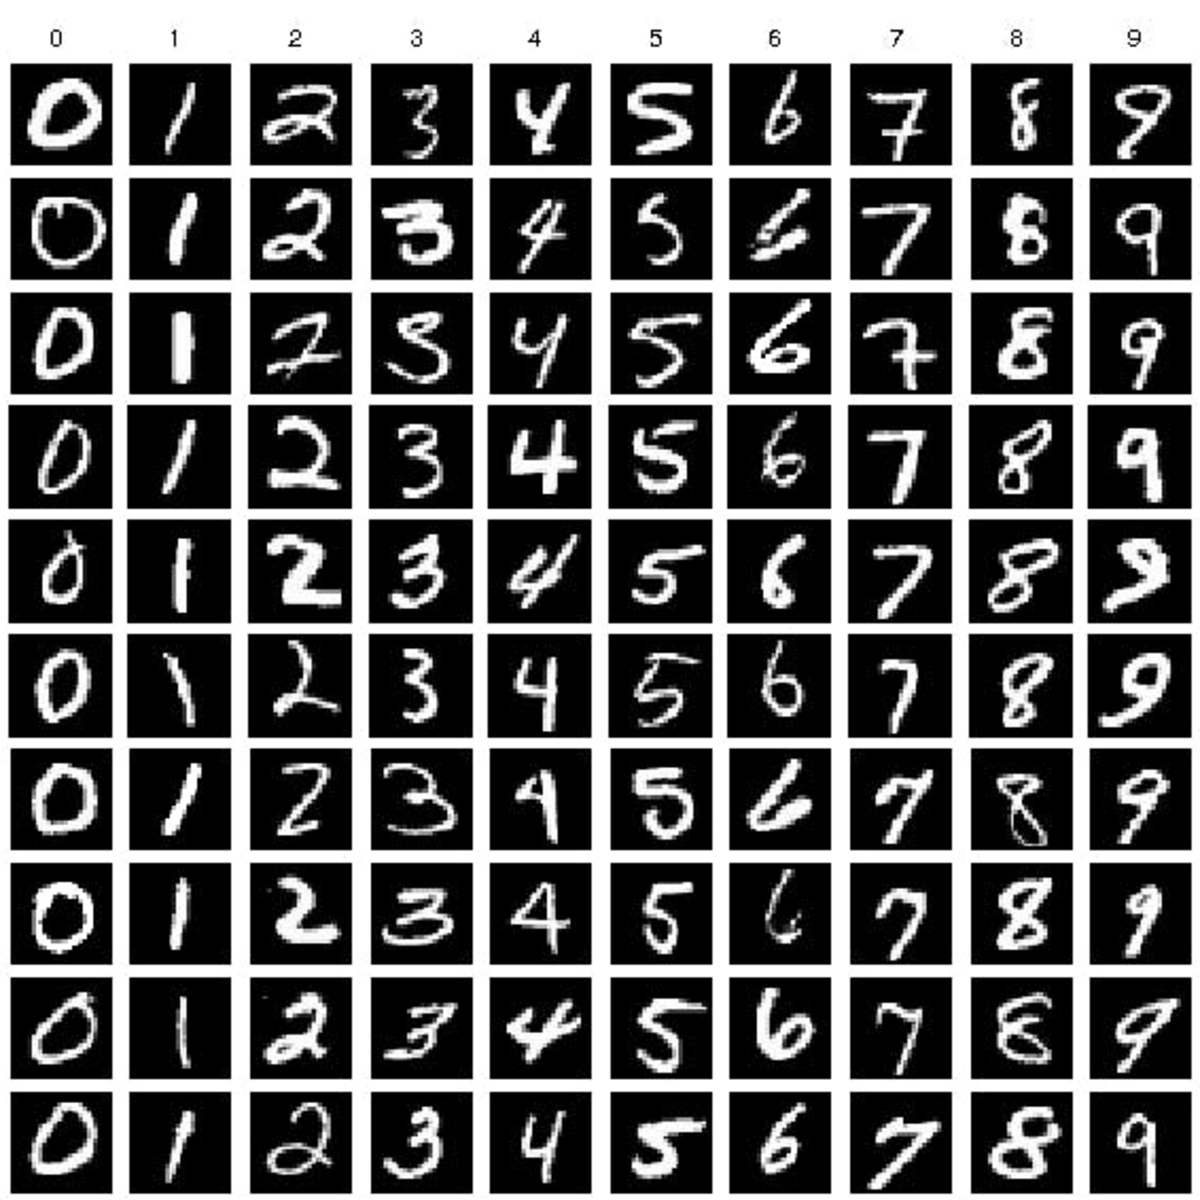
\includegraphics[width=0.75\textwidth]{sources/dataset-card.png}
    \caption{Mostres del conjunt de dades MNIST amb dígits manuscrits classificats.}
    \label{fig:mnist_dataset}
\end{figure}

Pel que fa al marc de treball d'intel·ligència artificial, tot i que TensorFlow i PyTorch dominen el mercat, s'ha seleccionat PyTorch \cite{pytorch_mnist_guide}. La seva flexibilitat en la gestió de grafs computacionals dinàmics proporciona una execució més àgil i un control estricte de la memòria, adaptant-se amb precisió a les limitacions dels nodes \textit{Edge}.

Finalment, l'arquitectura de la xarxa neuronal determina el grau d'exigència computacional. En lloc d'emprar un Perceptró Multicapa (MLP) bàsic, s'ha implementat una Xarxa Neuronal Convolucional (CNN). Aquesta decisió respon a la necessitat de simular un escenari real de visió per computador: les operacions matricials pròpies d'una CNN sotmeten a un estrès real la CPU i la RAM del dispositiu, garantint que l'experiment no només avalui la xarxa, sinó que mesuri l'impacte directe de l'arquitectura sobre una càrrega de càlcul intensiva.

\begin{figure}[H]
    \centering
    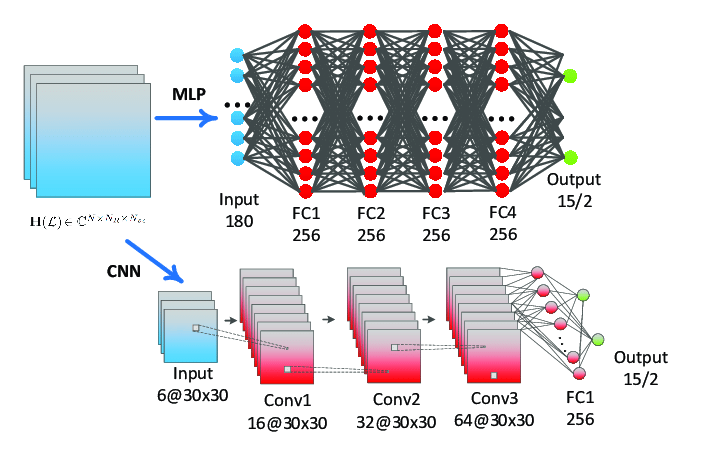
\includegraphics[width=0.85\textwidth]{sources/mlp_cnn_architecture.png}
    \caption{Arquitectura comparativa de xarxes MLP i CNN dissenyades per a tasques de classificació i regressió. Font: Adaptada de \cite{xiang2019robust}.}
    \label{fig:arquitectura_mlp_cnn}
\end{figure}

La Figura \ref{fig:arquitectura_mlp_cnn} il·lustra de manera conceptual l'estructura general d'una xarxa MLP i d'una CNN; les dimensions concretes hi són merament il·lustratives i no es corresponen amb l'arquitectura específica implementada en aquest treball, detallada al Capítol \ref{ch:implementation} (Listing \ref{lst:regex_extraction}).